\section{Πρώτη Φάση Πειραμάτων}
\label{sec:experiments_phase1}

Οι μετρήσεις κατανάλωσης ισχύος για τον επεξεργαστή Intel-i7-6700 έγιναν
χρησιμοποιώντας το εργαλείο \emph{PowerAPI} \cite{grant2016standardizing}.
Το τελευταίο, επιτρέπει την μέτρηση κατανάλωσης ισχύος σε
επίπεδο διεργασίας (process). Για την βέλτιστη λειτουργία του,
απαιτείται η ρύθμιση της παραμέτρου TDP (Thermal Design Power) του εκάστοτε
επεξεργαστή στον οποίο λαμβάνονται οι μετρήσεις. Η τιμή αυτής της παραμέτρου για τον επεξεργαστή
Intel-i7-6700, θεωρήθηκε στα 65W σύμφωνα με το αντίστοιχο τεχνικό εγχειρίδιο
\footnote{Intel i7 6700 TDP: \url{http://ark.intel.com/products/88196/Intel-Core-i7-6700-Processor-8M-Cache-up-to-4_00-GHz}}.
Επιπρόσθετα, για τις μετρήσεις που πραγματοποιήθηκαν λήφθηκαν υπόψη οι εξής παράγοντες:
\begin{itemize}
  \item{Δυναμική κατανάλωση ισχύος που οφείλεται στην δραστηριότητα των λογικών πυλών του επεξεργαστή}
  \item{Κατανάλωση ισχύος ανοικτού κυκλώματος (short-circuit)}
  \item{Απώλειες ισχύος λόγω διαρροής ρεύματος στα τρανζίστορ του επεξεργαστή (transistor leakage currents)}
\end{itemize}

Οι εκδόσεις των εργαλείων λογισμικού που χρησιμοποιήθηκαν
κατά την διάρκεια των πειραμάτων για τον επεξεργαστή Intel-i7-6700 είναι:
\begin{itemize}
  \item{Keras: v1.1.0}
  \item{Theano: v0.9.0-dev3}
  \item{numpy: v1.12.0}
  \item{scipy: v0.19.0-dev0}
\end{itemize}


% --------------------------------------------------------------------------

\subsection{AlexNet}

Οι παράμετροι των πειραμάτων είναι οι εξής:
\begin{itemize}
  \item{Αριθμός επαναλήψεων: 1000}
  \item{Αριθμός Νημάτων: 1, 2, 4, 8}
\end{itemize}

Στον \autoref{tab:alexnet_i7} παρουσιάζονται τα αποτελέσματα της μέσης τιμής
του χρόνου εκτέλεσης, ενώ στο \autoref{fig:alexnet_results_i7} φαίνεται
το διάγραμμα του χρόνου εκτέλεσης σε κάθε επανάληψη.

\begin{table}[H]
  \begin{center}
    \caption{Μετρήσεις πειραμάτων για το δίκτυο AlexNet σε επεξεργαστή Intel-i7-6700}
    \label{tab:alexnet_i7}
    \begin{tabular}{ | c | c | c | c | }
      \hline
      \rowcolor{Gray}
      \# νημάτων & Χρόνος Εκτέλεσης (sec) & Κατανάλωση Ισχύος (Watts) & Perf / Watt \\
      \hline
      1 & $0.117$ & $8.21$ & $1.04$ \\
      2 & $0.095$ & $16.43$ & $0.64$ \\
      4 & $0.095$ & $32.62$ & $0.32$ \\
      8 & $0.127$ & $58.84$ & $0.13$ \\
      \hline
    \end{tabular}
  \end{center}
\end{table}

Η μέγιστη τιμή μνήμης RAM που δεσμεύει το δίκτυο AlexNet μετρήθηκε στα \emph{692MB}.

\begin{figure}[H]
  \centering
  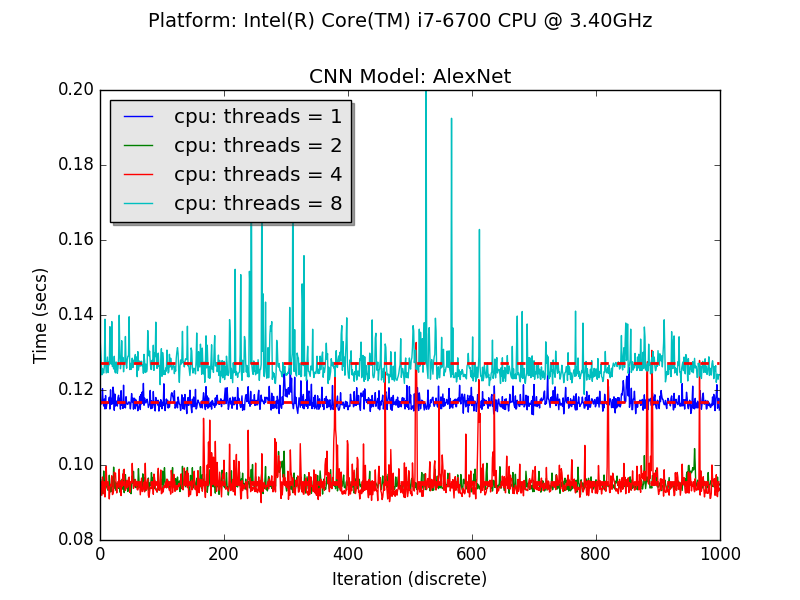
\includegraphics[width=0.8\textwidth]{./images/chapter6/benchmark_alexnet_i7.png}
  \caption[Χρόνoι εκτέλεσης για το δίκτυο AlexNet σε επεξεργαστή i7]{Χρόνοι εκτέλεσης για το δίκτυο AlexNet σε επεξεργαστή i7}
  \label{fig:alexnet_results_i7}
\end{figure}



%%----------------------------------------------------------------------------

\subsection{VGG16}

Οι παράμετροι των πειραμάτων είναι οι εξής:
\begin{itemize}
  \item{Αριθμός επαναλήψεων: 100}
  \item{Αριθμός Νημάτων: 1, 2, 4, 8}
\end{itemize}

Η μέσες τιμές του χρόνου εκτέλεσης των πειραμάτων παρουσιάζονται στον \autoref{tab:vgg16_i7}.
Η απαιτούμενη τιμή μνήμης RAM μετρήθηκε στα \emph{710MB}.

\begin{table}[H]
  \begin{center}
    \caption{Μετρήσεις πειραμάτων για το δίκτυο VGG16 σε επεξεργαστή Intel-i7-6700}
    \label{tab:vgg16_i7}
    \begin{tabular}{ | c | c | c | c | }
      \hline
      \rowcolor{Gray}
      \# νημάτων & Χρόνος Εκτέλεσης (sec) & Κατανάλωση Ισχύος (Watts) & Perf / Watt \\
      \hline
      1 & $0.7709$ & $8.26$ & $0.157$ \\
      2 & $0.5577$ & $15.78$ & $0.113$ \\
      4 & $0.4734$ & $29.75$ & $0.071$ \\
      8 & $0.6555$ & $58.97$ & $0.025$ \\
      \hline
    \end{tabular}
  \end{center}
\end{table}

\begin{figure}[H]
  \centering
  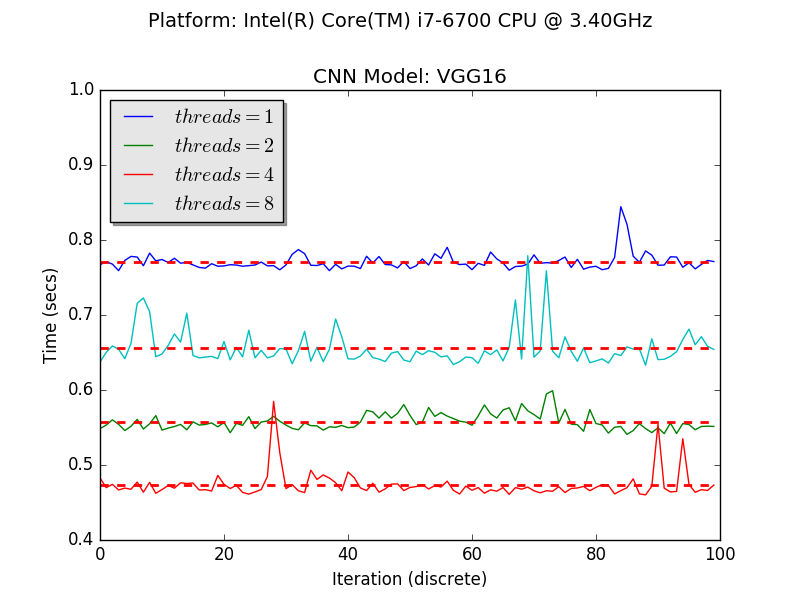
\includegraphics[width=0.8\textwidth]{./images/chapter6/benchmark_vgg16_i7.png}
  \caption[Χρόνoι εκτέλεσης για το δίκτυο VGG16 σε επεξεργαστή i7]{Χρόνοι εκτέλεσης για το δίκτυο VGG16 σε επεξεργαστή i7}
  \label{fig:vgg16_results_i7}
\end{figure}



%%----------------------------------------------------------------------------

\subsection{Tiny-YOLO}

Οι παράμετροι των πειραμάτων είναι οι εξής:
\begin{itemize}
  \item{Αριθμός επαναλήψεων: 1000}
  \item{Αριθμός Νημάτων: 1, 2, 4, 8}
\end{itemize}

Η αντίστοιχη μέση τιμή των χρόνων εκτέλεσης των πειραμάτων παρουσιάζονται στον \autoref{tab:yolo_i7}.
Σημαντικό να αναφερθεί ότι ο χρόνος εκτέλεσης της αντίστοιχης υλοποίησης της ερευνητικής ομάδας
που σχεδίασε το δίκτυο Tiny-YOLO, μετρήθηκε στα \emph{1.096 δευτερόλεπτα} (δεν χρησιμοποιούνται νήματα).

\begin{table}[H]
  \begin{center}
    \caption{Μετρήσεις πειραμάτων για το δίκτυο Tiny-YOLO σε επεξεργαστή Intel-i7-6700}
    \label{tab:yolo_i7}
    \begin{tabular}{ | c | c | c | c | }
      \hline
      \rowcolor{Gray}
      \# νημάτων & Χρόνος Εκτέλεσης (sec) & Κατανάλωση Ισχύος (Watts) & Perf / Watt \\
      \hline
      1 & $0.1871$ & $8.23$ & $0.65$ \\
      2 & $0.1609$ & $16.39$ & $0.38$ \\
      4 & $0.1516$ & $32.7$ & $0.2$ \\
      8 & $0.2309$ & $61.17$ & $0.07$ \\
      \hline
    \end{tabular}
  \end{center}
\end{table}

Η μνήμη (μέγιστη) που απαιτείται κατά την διαδικασία
προς-τα-εμπρός εκτέλεσης μετρήθηκε στα \emph{379MB}.

\begin{figure}[H]
  \centering
  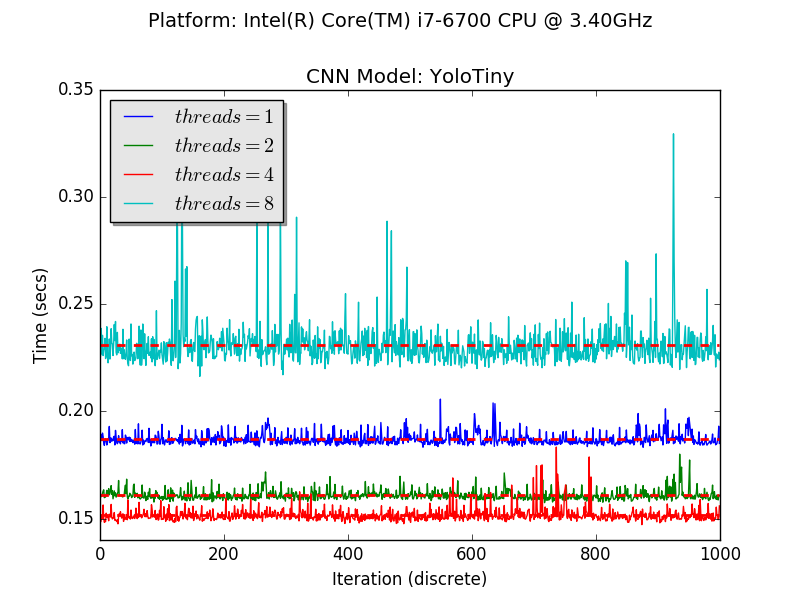
\includegraphics[width=0.8\textwidth]{./images/chapter6/benchmark_yolotiny_i7.png}
  \caption[Χρόνoι εκτέλεσης για το δίκτυο Tiny-YOLO σε επεξεργαστή i7]{Χρόνοι εκτέλεσης για το δίκτυο Tiny-YOLO σε επεξεργαστή i7}
  \label{fig:yolotiny_results_i7}
\end{figure}


